\documentclass[11pt]{article}

\usepackage{times}
\usepackage[utf8]{inputenc} % allow utf-8 input
\usepackage[T1]{fontenc}    % use 8-bit T1 fonts
\usepackage{url}            % simple URL typesetting
\usepackage{graphics}
\usepackage{color}
\usepackage{amsfonts}       % blackboard math symbols
\usepackage{amsmath}       % blackboard math symbols
\usepackage{amssymb}

\usepackage{lipsum}

\usepackage{tikz}
\usetikzlibrary{angles,quotes,calc}

\usepackage{geometry}
\geometry{left=2.8cm,right=2.8cm,top=2.6cm,bottom=2.6cm}
\usepackage{fancyhdr}
\pagestyle{fancy}
\usepackage{hyperref}% should be the last package you include

\newcommand{\theteam}{}
\newcommand{\team}[1]{\def\theteam{#1}}


\fancyhead[L]{\theteam}
\fancyhead[R]{\thepage}
\cfoot{}

\setlength{\parindent}{0pt}

\team{WayneGradientzky: Rajinish Aneel Bhatia, Bartol Markovinović, Mohd Khizir Siddiqui}
\title{RL-Course 2025/26: Final Project Report}
\author{\theteam}

\begin{document}
\maketitle

\section{Introduction}\label{sec:intro}

\section{Method}\label{sec:Method}
\subsection{SAC}

\subsection{Twin Delayed Deep Deterministic Policy Gradient (TD3)}
Twin Delayed Deep Deterministic Policy Gradient (TD3)\cite{fujimoto2018:TD3} is a model-free, off-policy deep reinforcement learning algorithm used for continuous action spaces. It was proposed as an improvement over Deep Deterministic Policy Gradient (DDPG) and addresses several failure modes of DDPG, by introducing clipped double Q-learning, delayed policy update, and target policy smoothing.

TD3 achieves this by maintaining two Q-networks ($Q_{\phi_1}$ and $Q_{\phi_2}$) and using their min as the TD target:
\label{td_target}\[
y = r + \gamma \min_{i=1,2}{Q_{\phi_{i}'}(s', \tilde{a})}
\quad (1)
\]
where $Q_{\phi_{i}'}$ is the corresponding target network, and $\tilde{a}$ is the action given by the policy $\pi_{\theta}$ pertubed by some noise:
\[
\tilde{a} = \pi_{\theta'}(s') + \epsilon,
\hspace{5mm}
\epsilon \sim \texttt{clip}(\mathcal{N}(0, \sigma), -c, c)
\]
The critic loss is defined as the expectation of mean squared Bellman error and each critic minimizes this:
\[
\mathcal{L}(\phi_i) = \mathbb{E}_{(s, a, r, s') \sim \mathcal{D}}(Q_{\phi_i}(s, a) - y)^2
\]
And the actor aims to maximize Q-values predicted by the first critic:
\[
J(\theta) = \mathbb{E}_{s \sim \mathcal{D}} Q_{\phi_1}(s, \pi_{\theta}(s))
\]

Unlike DDPG, TD3 updates the actor and target networks less frequently than the critics. In our project the actor updates every 2 steps a critic steps.

\subsubsection{Custom Opponent And Bank-shot reward}
We noticed early on that the model did not always manage to learn ricochet (bank) shots, so in order to help it better defend against opponents that hit bank shots we introdued a hard coded opponent that always hits such bank shots.

\begin{center}
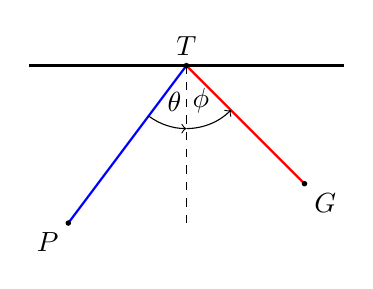
\begin{tikzpicture}[scale=0.5]

% ---- Coordinates ----
\coordinate (P) at (-3,-2);   % puck
\coordinate (G) at (3,-1);    % goal
\coordinate (T) at (0,2);     % impact point
\coordinate (W1) at (-4,2);
\coordinate (W2) at (4,2);
\coordinate (N) at (0,-2);    % point to define normal direction

% ---- Wall ----
\draw[thick] (W1) -- (W2);
% \node[above] at (0,2) {Wall};

% ---- Rays ----
\draw[thick, blue] (P) -- (T);
\draw[thick, red] (T) -- (G);

% ---- Normal (middle line) ----
\draw[dashed] (T) -- (N);

% ---- Points ----
\fill (P) circle (2pt) node[below left] {$P$};
\fill (G) circle (2pt) node[below right] {$G$};
\fill (T) circle (2pt) node[above] {$T$};

% ---- Angle theta (blue to normal) ----
\pic [
    draw,
    ->,
    angle radius=0.8cm,
    "$\theta$"
] {angle = P--T--N};

% ---- Angle phi (normal to red) ----
\pic [
    draw,
    ->,
    angle radius=0.8cm,
    "$\phi$"
] {angle = N--T--G};

\end{tikzpicture}
\end{center}

If we take $P$ as the position of the puck, $G$ as the position of the goal, and $T$ as the target we must shoot at to reach $G$. Then $T_y$ is known because that is the boundary and we only need to find $T_x$. We can assume that $T_x \ge P_x$ and $G_x \ge T_x$. We can also deduce that: 
\[
\tan(\theta) = \frac{|T_y - P_y|}{T_x - P_x}
\hspace{5mm}
\tan(\phi) = \frac{|T_y - G_y|}{G_x - T_x}
\]

If we assume frictionless walls then $\theta = \phi$ and we get that:
\[
{T_x} = \frac{|T_y - P_y|G_x +  |T_y - G_y|P_x}{{|T_y - G_y| + |T_y - P_y|}}
\]

This agent has rougly $94\%$ win rate against the provided weak opponent and $80\%$ win rate against the strong opponent. We also used similar logic for rewarding the agent if it shoots in this direction to make it prefer these shots.

\subsubsection{N-step returns}
Instead of using the TD target defined in (1) which can propagate reward signal slowly, since each update step only looks one step ahead. We use the generalized n-step returns which can significantly speed up learning:
\[
y = r(s_0) + \gamma r(s_1) + \dots + \gamma^{n-1} r(s_{n-1}) + \gamma^n q(s_n, \tilde{a})
\]

\subsubsection{Layer Norm}
Layer normalization normalizes the inputs accross the feature dimension for each sample independently. For a given input, layer norm computes:
\[
\texttt{LayerNorm(x)} = \frac{\texttt{x} - \mu}{\sigma + \epsilon}\gamma + \beta
\]
In the context of reinforcement learning, layer normalization has been shown to stablize training by reducing sensitivity to the scale of inputs and gradients. We apply layer norm after each linear layer in both actor and critic networks.

\subsubsection{Pink Noise}
To induce exploration we add some noise to the action chosen by the policy: $a(s(t)) = \pi_{\theta}(s_t) + \epsilon_t$. Most commonly, Gaussian noise with an annealed standard deviation is used. Eberhard et al.~\cite{eberhard2023pink} showed that pink noise or $1/f$ noise can improve exploration because pink noise is temporally correlated and produces action sequences that are not too jittery compared to white noise. In our experiments we anneal the standard deviation of the noise over training, starting with higher exploration and gradually reducing it as the policy matures.


\subsection{TDMPC}

\section{Evaluation}\label{sec:eval}
\subsection{SAC}

\subsection{TD3}
\subsubsection{Training in phases (Opponent Scheduling)}
The model was trained in phases: the first phase involved just training against the Weak Opponent provided with the environment, in the second phase an opponent from Weak Opponent and Strong opponent was chosen probabilistically with the corresponding probabilities being $30\%$ and $70\%$. In the final phase the opponents were again chosen probabilistically: $20\%$ for weak opponent, $20\%$ for strong opponent, $10\%$ for custom opponent and $50\%$ from a pool of past checkpoints. An adaptive technique like Thompson sampling for automatically choosing the opponents did not seem to work well as shown in the figures below:

\begin{figure}[h]
    \centering
    \begin{minipage}{0.48\textwidth}
        \centering
        \includegraphics[width=\textwidth]{td3_images/baseline1.png}
        \caption{Winrate (trained in phases)}
        \label{fig:baseline}
    \end{minipage}
    \hfill
    \begin{minipage}{0.48\textwidth}
        \centering
        \includegraphics[width=\textwidth]{td3_images/thompson.png}
        \caption{Winrate (trained using Thompson sampling)}
        \label{fig:thompson}
    \end{minipage}
\end{figure}

\subsubsection{Self-Play}
Self play was the part of the third phase of training and was implemented by keeping a queue of $50$ checkpoints and adding a new checkpoint every $50000$ timesteps. This ensured that the model had enough learning experience from each of its previous checkpoints to be able to defeat them.

\subsubsection{LayerNorm}
While LayerNorm seemed to converge much earlier for strong and weak bot, it seemed to have problems generalizing when it came to self play. We observed it making draws over time with all of its previous checkpoints.

\begin{figure}[h]
    \centering
    \begin{minipage}{0.48\textwidth}
        \centering
        \includegraphics[width=\textwidth]{td3_images/baseline_vs_ln.png}
        \caption{Winrate of baseline and layer norm}
        \label{fig:bs_v_ln}
    \end{minipage}
    \hfill
    \begin{minipage}{0.48\textwidth}
        \centering
        \includegraphics[width=\textwidth]{td3_images/ln_draw_rate.png}
        \caption{Draw rate of layer norm against previous checkpoints}
        \label{fig:ln_draw_rate}
    \end{minipage}
\end{figure}

\subsubsection{Environment Scheduling}
Environment Scheduling was introduced in the 3rd phase of training with $30\%$ in attack mode and $70\%$ in defense mode to improve the defending skills of the agent.

\begin{figure}[h]
    \centering
    \begin{minipage}{0.48\textwidth}
        \centering
        \includegraphics[width=\textwidth]{td3_images/n_step_results.png}
        \caption{Winrate against previous checkpoints}
        \label{fig:n_steps_result}
    \end{minipage}
    \hfill
    \begin{minipage}{0.48\textwidth}
        \centering
        \includegraphics[width=\textwidth]{td3_images/right_possesion_win_rate.png}
        \caption{Winrate (opponent started first)}
        \label{fig:right_possesion_winrate}
    \end{minipage}
\end{figure}


\begin{figure}[h]
    \centering
    \begin{minipage}{0.48\textwidth}
        \centering
        \includegraphics[width=\textwidth]{td3_images/heatmapnormal.png}
        \caption{Puck Density With Normal Reward}
        \label{fig:normal_reward}
    \end{minipage}
    \hfill
    \begin{minipage}{0.48\textwidth}
        \centering
        \includegraphics[width=\textwidth]{td3_images/heatmapbank_pref.png}
        \caption{Puck Density With Bank Shot Preference Reward}
        \label{fig:bank_pref_reward}
    \end{minipage}
\end{figure}


\subsection{TDMPC}

\section{Discussions and Conclusion}\label{sec:conclusion}

\bibliographystyle{abbrv}
\bibliography{main}

\end{document}
